\section{Introduction}

Students learn by practicing many problems, but generating fresh problems that have specific characteristics, such as using a certain set of concepts or being of a given difficulty level, is a tedious task for a teacher. Our goal is to automatically generate programming
problems that are parameterized by complexity and by the set of
concepts a student wants to learn. In this work, we present $\puzzlejar$, a system
that solves a simpler task of automatically generating
Sudoku and Fillomino puzzles of different complexity levels. Our
technique and algorithms are general enough to generate programming
problems as well as problems from other domains including algebra and
trigonometry problems.

We present a generic iterative constraint-based algorithm for
generating problems of different complexity levels. Most previous
approaches for automatically generating puzzle problems have been
specific to a given puzzle and are based on a set of heuristic
rules. $\puzzlejar$, on the other hand, lets one specify the puzzle
definition and puzzle complexity in a declarative fashion using
constraints and then uses efficient constraint-solving to
incrementally solve constraints generated from different
iterations. The system first generates a completely random problem
that satisfies the constraints. It then removes elements from the
complete problem using a user-defined probabilistic function such that
certain validity constraints are satisfied. We use the z3 SMT
solver~\cite{z3} and its theory of linear arithmetic for representing
and solving the constraints.

We have successfully used $\puzzlejar$ to automatically generate more
than 200,000 9x9 Sudoku puzzles and more than 10,000 Fillomino
puzzles. A random 9x9 Sudoku and Fillomino puzzle automatically
generated by our system is shown in Figure.~\ref{Sudokuprobsol} and
Figure.~\ref{Fillominoprobsol} respectively. Our puzzles vary across a
number of features: number of empty spaces, number of solutions,
distribution of empty spaces, repetition of digits etc. The
declarative nature of $\puzzlejar$ lets us easily parameterize the
algorithm to also generate puzzles of different sizes, such as 16x16
and 25x25 Sudoku puzzles. Since computing the difficulty level of a
Sudoku puzzle or a Fillomino puzzle is still an open research problem,
we resort to machine learning techniques to learn a function over the
puzzle features from a set of labelled Sudoku problems obtained from
popular Sudoku websites and newspapers. We then use this learnt
function to characterize the Sudoku problems generated by our system
into different complexity levels. We are currently extending our
system to support generation of Python programming problems and other
puzzles.

\begin{figure}[!htpb]
\centering
\begin{tabular}{c c}
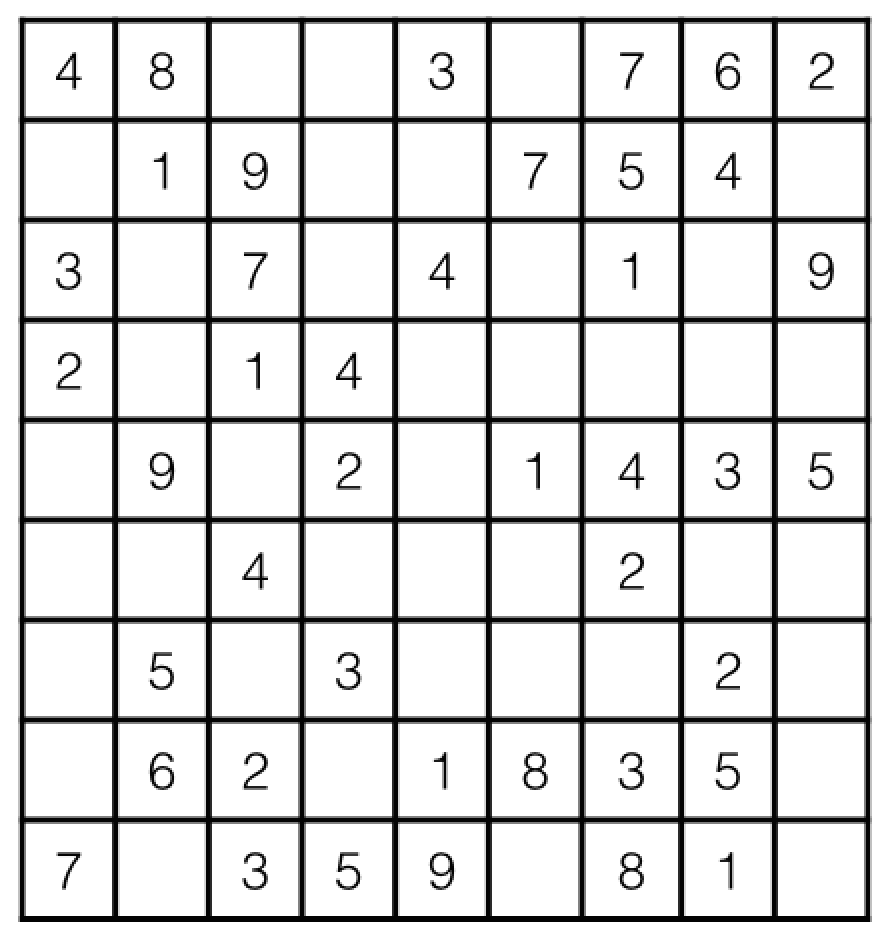
\includegraphics[scale=0.40]{puzzlefigs/sudoku_prob.png}
&
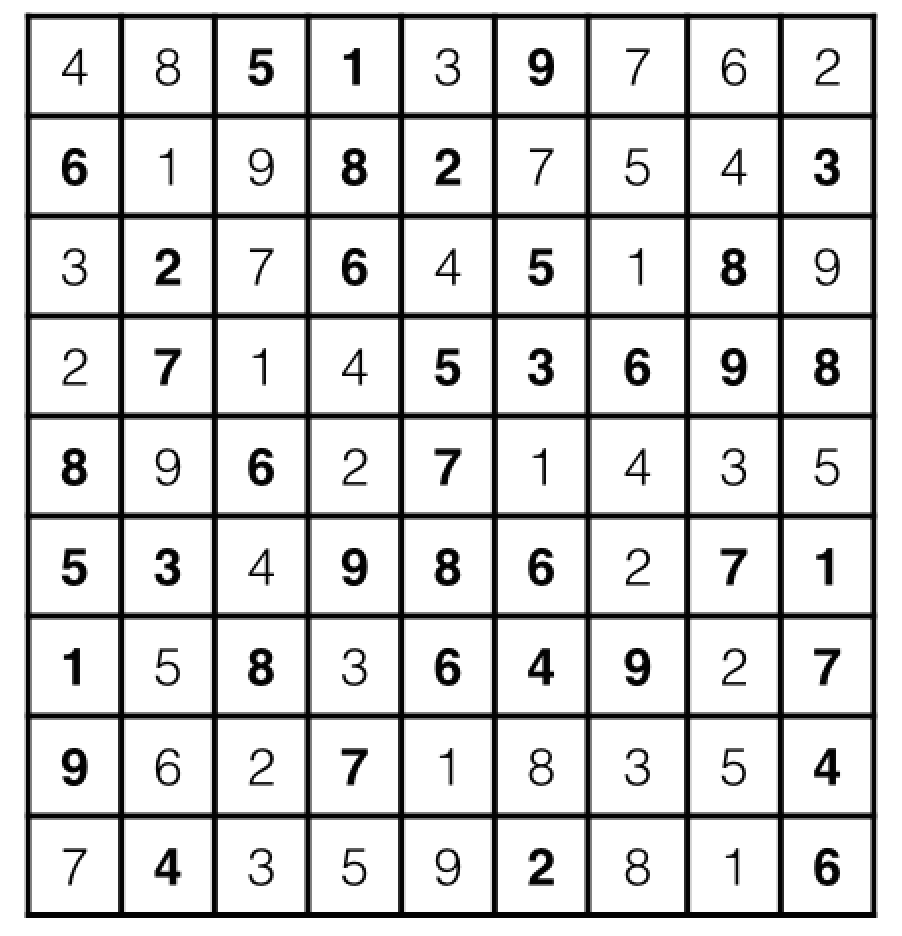
\includegraphics[scale=0.40]{puzzlefigs/sudoku_sol.png}
\\
(a) & (b)
\end{tabular}
\caption{(a) A 9x9 Sudoku problem automatically generated by our system, and (b) its solution.}
\label{Sudokuprobsol}
\end{figure}


\begin{figure}[!htpb]
\centering
\begin{tabular}{c c}
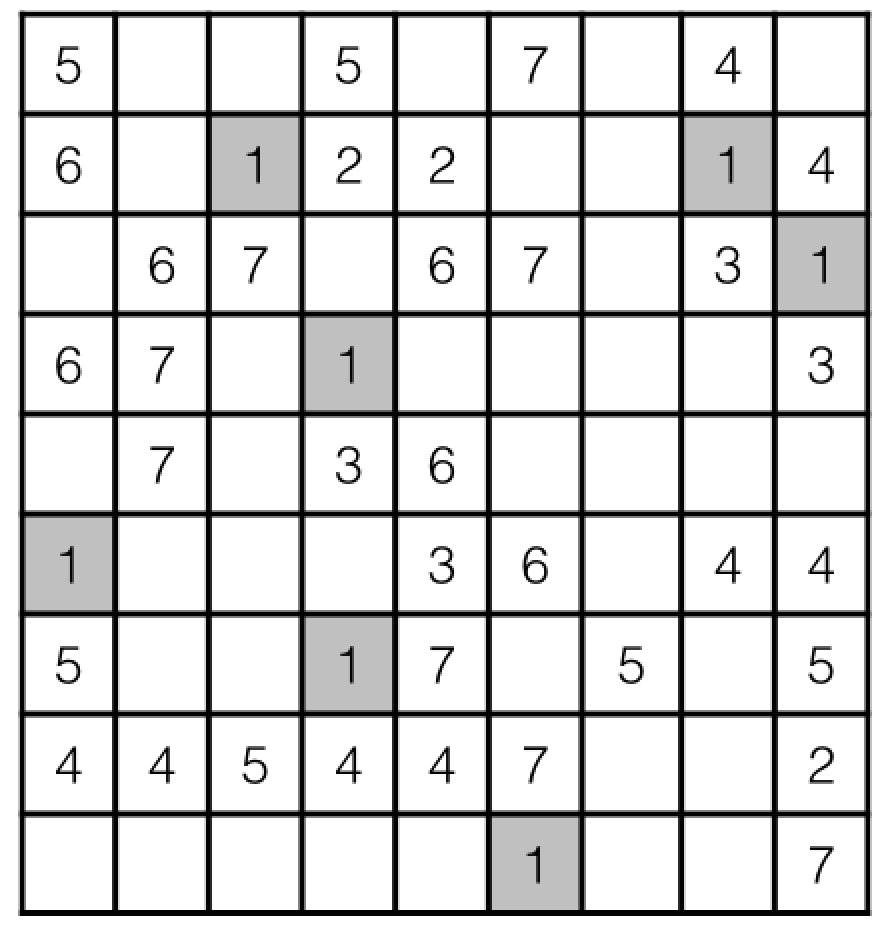
\includegraphics[scale=0.40]{puzzlefigs/fillomino_prob.png}
&
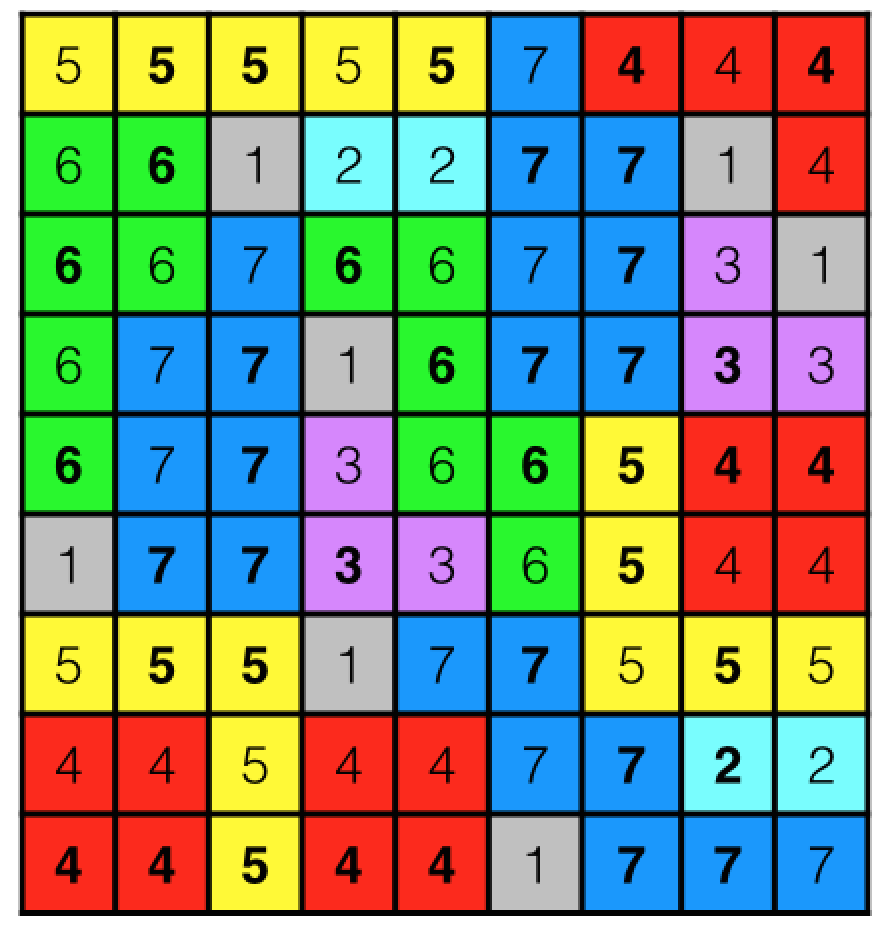
\includegraphics[scale=0.40]{puzzlefigs/fillomino_sol.png}
\\
(a) & (b)
\end{tabular}
\caption{(a) A 9x9 Fillomino problem automatically generated by our system, and (b) its solution.}
\label{Fillominoprobsol}
\end{figure}

This paper makes the following major contributions:

\begin{itemize}
\item We present a general constraint-based system, $\puzzlejar$, to automatically generate puzzles of varying complexity.
\item We present a machine learning approach to learn the
  complexity function of puzzles.
\item We successfully evaluate the $\puzzlejar$ system to generate
  more than $200,000$ Sudoku puzzles and $10,000$ Fillomino puzzles of
  different complexity.
\item We have created an interactive website to let users solve these
  puzzles. To the best of our knowledge, the number of Sudoku and
  Fillomino puzzles are at least an order of magnitude more than the
  puzzles present on any website/book.
\end{itemize}
